% ============================================================================
%  EXPERIMENT SETUP -- drop-in section for the ASIA CCS / ACM CCS paper.
%
%  Assumptions made while writing this (check before using):
%    - Placed after Method, before Results/Discussion. Defines \label{sec:eval},
%      which \ref{sec:eval} in VLI_threat_model_en.tex, VLI_collapse_mechanism_en.tex
%      and VLI_method_en.tex already points at.
%    - Every number below was read off the actual run logs, not assumed:
%      the six files in Experiment_Result/ (VLIstar_Fig1a/b/c, VLIstar_Table1
%      [two variants], VLIstar_Table2) and log_vgg16_lr0.01.txt /
%      log_vgg16_lr0.05.txt. Re-grep the "Namespace(...)" and "loaded global
%      model checkpoint" lines of those files before changing any value here.
%    - Table~\ref{tab:exhibits} names the six exhibits after their source
%      files' own prefixes (Fig1a/b/c, Table1, Table1-singlestep, Table2); if
%      the final paper numbers figures/tables differently, update the first
%      column only.
%    - The main comparison (Table 1, VGG16/CIFAR10) is pinned to lr$=0.05$,
%      not the codebase's default lr$=0.01$: with lr$=0.01$ RLU's own attack
%      falls far below its published 80--83\% iAcc range on this
%      architecture, while lr$=0.05$ reproduces it (log_vgg16_lr0.05.txt vs.
%      log_vgg16_lr0.01.txt). We therefore do not use the older
%      VLIstar_Table1_10_local_epochs_VGG16_CIFAR10.txt (lr$=0.01$,
%      checkpoint acc 89.33) for Table 1; log_vgg16_lr0.05.txt (checkpoint
%      acc 86.75) is the source of record.
%    - Uses $m$, $B$, $n=mB$, $C$, $N_j$, $\widehat N_j$ exactly as defined
%      in Section~\ref{sec:prelim}; do not reintroduce batch\_size/local\_epochs
%      as prose variable names.
%    - cAcc and irec are transcribed directly from
%      Client.accuracy\_calculation (client/client\_base.py); irec is the
%      same quantity main.py's top-level loop calls iAcc (and RLU's own
%      paper calls iAcc) -- one metric, three names across three documents.
%      We keep "irec" as the paper's name, matching every earlier section.
%    - Section~\ref{sec:eval-rq2} (RQ2) needs \usepackage{graphicx},
%      \usepackage{subcaption}, and \usepackage{multirow} in addition to
%      the packages VLI_preliminaries_en.tex already assumes (amsmath/
%      amssymb, array, booktabs). Its figure is three separate files --
%      figures/fig1a_svhn.png, fig1b_cifar10.png, fig1c_cifar100.png --
%      laid out as a row of subfigures. Each panel's matplotlib style is
%      copied parameter-for-parameter from the user's own
%      figure/Line_chart.py (figsize 7x7, fontsize 20, markersize 10,
%      linewidth 3.5, dashed grid, spine width 2, box_aspect 0.8, legend
%      OUTSIDE the axes via bbox_to_anchor=(1.02,1)) plus that same
%      file's commented-out "CHUA TRAINED DEN DA TRAINED" convention
%      (x-axis = global round, black dashed Model-Accuracy overlay,
%      marker 'H', linestyle (0,(5,3))), now actually enabled. Do not
%      swap in the plain/no-grid/inside-legend look of RLU's own printed
%      Figure 1 (figure1_page7.png) -- that was an earlier, rejected
%      draft of this figure. Regenerated by
%      scripts/plot_fig1_linechart_style.py from scripts/parse_rq2.py's
%      output over Experiment_Result/ -- re-run both if any underlying
%      log changes, do not hand-edit the numbers or the PNGs directly.
% ============================================================================

\section{Experiment Setup}
\label{sec:eval}

\subsection{Research questions}
\label{sec:eval-rq}

Section~\ref{sec:collapse} argues, and in part proves, that iLRG,
LLG\(^+\), ZLG\(^+\), and RLU degrade for a specific structural reason --
a fixed, auxiliary-derived center that does not shrink along with the
gradient -- rather than only because the gradient signal itself shrinks.
Section~\ref{sec:method} builds \ourmethod{} to avoid that dependence
entirely. The experiments below are organized around two questions:

\begin{description}
\item[RQ1 (mechanism).] Does the degradation these four baselines
actually show as the attacked model converges match what
Theorem~\ref{thm:collapse} and its branch-specific arguments
(Section~\ref{sec:collapse}) predict -- drift toward a fixed center $c$,
not toward the zero vector -- rather than some other failure their own
papers have not isolated? Figure~1 reports irec/cAcc against
measured training accuracy for exactly this purpose, and
\texttt{--collapse\_diag}/\texttt{--rlu\_diag}/\texttt{--inspect}
(Section~\ref{sec:collapse}) instrument the quantities the proof is
stated in terms of ($\|G\|_1$, the residual $R$, the drift from $c$)
directly, rather than only their downstream effect on irec.

\item[RQ2 (comparison).] Across the datasets, architectures, and
partition skews of Table~\ref{tab:exhibits}, how does \ourmethod{}'s
irec/cAcc compare to the four baselines -- in particular in the
high-accuracy regime where RQ1's mechanism predicts the baselines should
fail but \ourmethod{}, having no auxiliary-derived center to drift
toward, should not? Tables~1 and~2 and the converged end of Figure~1
answer this directly; the ablations of
Section~\ref{sec:method-oracle} further decompose \ourmethod{}'s own
error into the two idealizations (uniform $Q$, $r\equiv1$) its closed
form makes, so a gap from RQ2 can be attributed to a specific assumption
rather than left as an unexplained residual.
\end{description}

\subsection{Datasets, models, and federated setup}
\label{sec:eval-setup}

We evaluate on four image classification datasets spanning $C=10$ to
$C=100$ classes and three architectures, federated across $10$ clients
with full participation (sampling rate $1$) under FedAvg. Each client's
partition is drawn once from a Dirichlet distribution of concentration
$\alpha$ over the $C$ classes~\cite{hsu2019dirichlet}; smaller $\alpha$
yields a more skewed, more non-IID partition. The attacker's auxiliary
set, when a baseline uses one (Section~\ref{sec:threat}), is a $10\%$
per-class sample of the \emph{test} split, held out from every client's
training data. Table~\ref{tab:exhibits} lists the six exhibits this
produces and the configuration behind each.

\begin{table}[t]
\centering
\caption{Dataset/model/partition configuration behind each exhibit. $B$ is
the batch size, $m$ the window length in local steps
(Section~\ref{sec:prelim-notation}).}
\label{tab:exhibits}
\footnotesize
\setlength{\tabcolsep}{3pt}
\begin{tabular}{@{}l l l c c c@{}}
\toprule
Exhibit & Dataset & Model & $C$ & $\alpha$ & $B$,\,$m$ \\
\midrule
Fig.~1a & SVHN & MobileNetV2 & 10 & 0.5 & 32, 10 \\
Fig.~1b & CIFAR-10 & ResNet18 & 10 & 0.5 & 64, 10 \\
Fig.~1c & CIFAR-100 & ResNet18 & 100 & 0.1 & 256, 10 \\
Table~1 & CIFAR-10 & VGG16 & 10 & 0.5 & 64, 10 \\
Table~1 (single-step) & CIFAR-10 & ResNet18 & 10 & 0.5 & 64, 1 \\
Table~2 & MNIST & MobileNetV2 & 10 & 0.05 & 64, 10 \\
\bottomrule
\end{tabular}
\end{table}

Table~2's $\alpha=0.05$ is deliberately extreme (most clients see only a
handful of classes) and stress-tests every estimator's behaviour at the
sparse end of Section~\ref{sec:method}'s design assumption; every other
exhibit uses a moderate skew ($\alpha \in \{0.1, 0.5\}$) representative of
the non-IID regime the baselines themselves evaluate on.

\subsection{Global model checkpoints}
\label{sec:eval-checkpoints}

Each dataset/model pair is pretrained with the same FedAvg loop and the
same per-step SGD configuration (momentum $0$, no weight decay is applied
to the step we read\footnote{\texttt{--weight\_decay} is parsed but not
passed to \texttt{torch.optim.SGD} in the code path used here.}) that is
later used for the attacked window, so a checkpoint's own training
trajectory is representative of what the attacker observes. Checkpoints
are saved every few rounds and named by their training-set top-1 accuracy
and round index.

Figure~1 (exhibits 1a--1c) attacks the \emph{entire} saved trajectory of
one dataset/model pair, from the first round (training accuracy within a
few points of the $1/C$ random baseline) to a converged checkpoint
(87--95\% depending on the pair): this is what lets Figure~1 plot recovery
against model accuracy rather than reporting it at one point. Tables~1
and~2 instead fix a single, well-converged checkpoint per dataset/model
pair ($86.75\%$ for VGG16/CIFAR-10, $87.36\%$ for the single-step
ResNet18/CIFAR-10 variant, $98.16\%$ for MobileNetV2/MNIST), matching the
paper's stated setting: a model the client population has already trained
to convergence, not one still at its first few rounds.

\subsection{Attack configuration}
\label{sec:eval-attack}

Every attack reads one client's accumulated final-layer gradient over a
window of $m$ local steps of batch size $B$ ($n=mB$ examples per window,
Section~\ref{sec:prelim-notation}); a client's stream is swept window by
window, non-overlapping, until its partition is exhausted. $m=10$
throughout except the single-step variant of Table~1 ($m=1$), which
isolates the setting the \texttt{RLG}-style literature itself emphasizes:
one SGD step per report, the minimum amount of accumulation a real
aggregator would ever see. RLU is the only baseline whose estimator reads
the learning rate directly (Section~\ref{sec:threat}); we use its own
learning rate ($\mathrm{lr}=0.05$ for Table~1's VGG16/CIFAR-10 run,
$\mathrm{lr}=0.01$ elsewhere) as the value supplied to that estimator, so
no baseline is run with a rate it was not also given.

\subsection{Metrics}
\label{sec:eval-metrics}

For one window, let $N_j$ be the true count of class $j$ and $\widehat
N_j$ the attacker's recovered count. We report two statistics of this
window, each then averaged uniformly over all windows of a client and
uniformly over the $10$ clients -- never weighted by partition size, so
one client's result counts the same as any other's:

\[
\mathrm{cAcc} = \frac1C\sum_{j=1}^C \mathbb{1}\bigl[\mathbb{1}[\widehat
N_j>0] = \mathbb{1}[N_j>0]\bigr],
\qquad
\mathrm{irec} = \frac1n\sum_{j=1}^C \min(\widehat N_j, N_j).
\]

\textsc{cAcc} is the fraction of classes whose \emph{presence} the
attacker gets right, independent of count; it is $1$ for an attacker that
recovers only the support of the window, even with every count wrong, and
it is what Section~\ref{sec:method-gstar}'s sparsity trade-off is stated
in terms of. \textsc{irec} is the histogram-intersection between the true
and recovered count vectors, normalized by the window size $n=\sum_j
N_j$; it is $1$ only when $\widehat N_j=N_j$ for every class, and it is
the metric we treat as primary throughout this paper, since cAcc alone
cannot distinguish a correct count from a correct guess at presence. Both
are bounded in $[0,1]$ and computed per window before any averaging, so a
window with few classes present is not implicitly down-weighted relative
to one with many. \textsc{irec} is the quantity this codebase's top-level
driver (\texttt{main.py}) calls \textsc{iAcc}, and the same quantity
RLU's own paper reports as \textsc{iAcc}; we keep the name \textsc{irec}
throughout this paper for consistency with
Sections~\ref{sec:threat}--\ref{sec:method}, and note the correspondence
here rather than silently switching names between sections.

\subsection{RQ2: comparison across datasets, architectures, and partition
skew}
\label{sec:eval-rq2}

\begin{figure*}[t]
\centering
\begin{subfigure}[b]{0.32\textwidth}
\centering
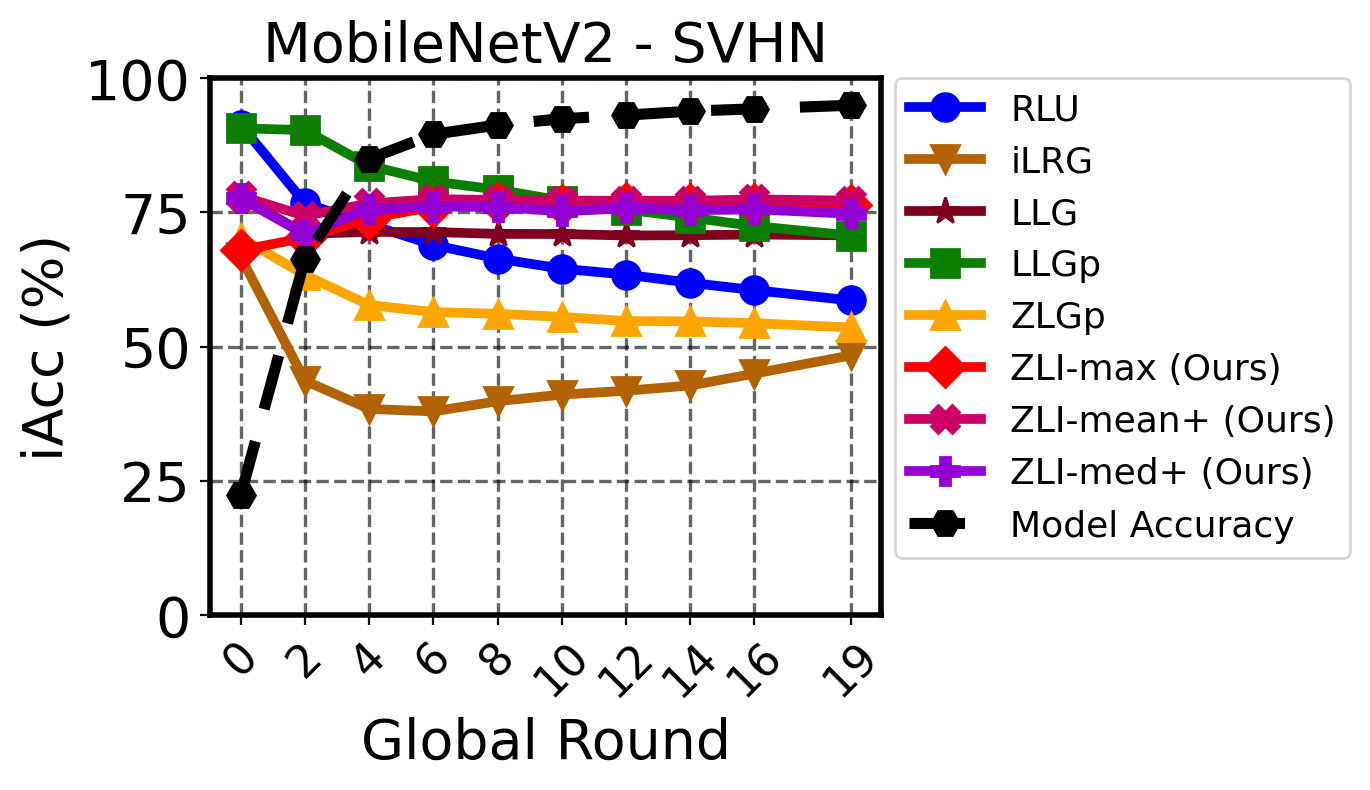
\includegraphics[width=\textwidth]{figures/fig1a_svhn.png}
\caption{}
\label{fig:rq2-sweep-a}
\end{subfigure}
\hfill
\begin{subfigure}[b]{0.32\textwidth}
\centering
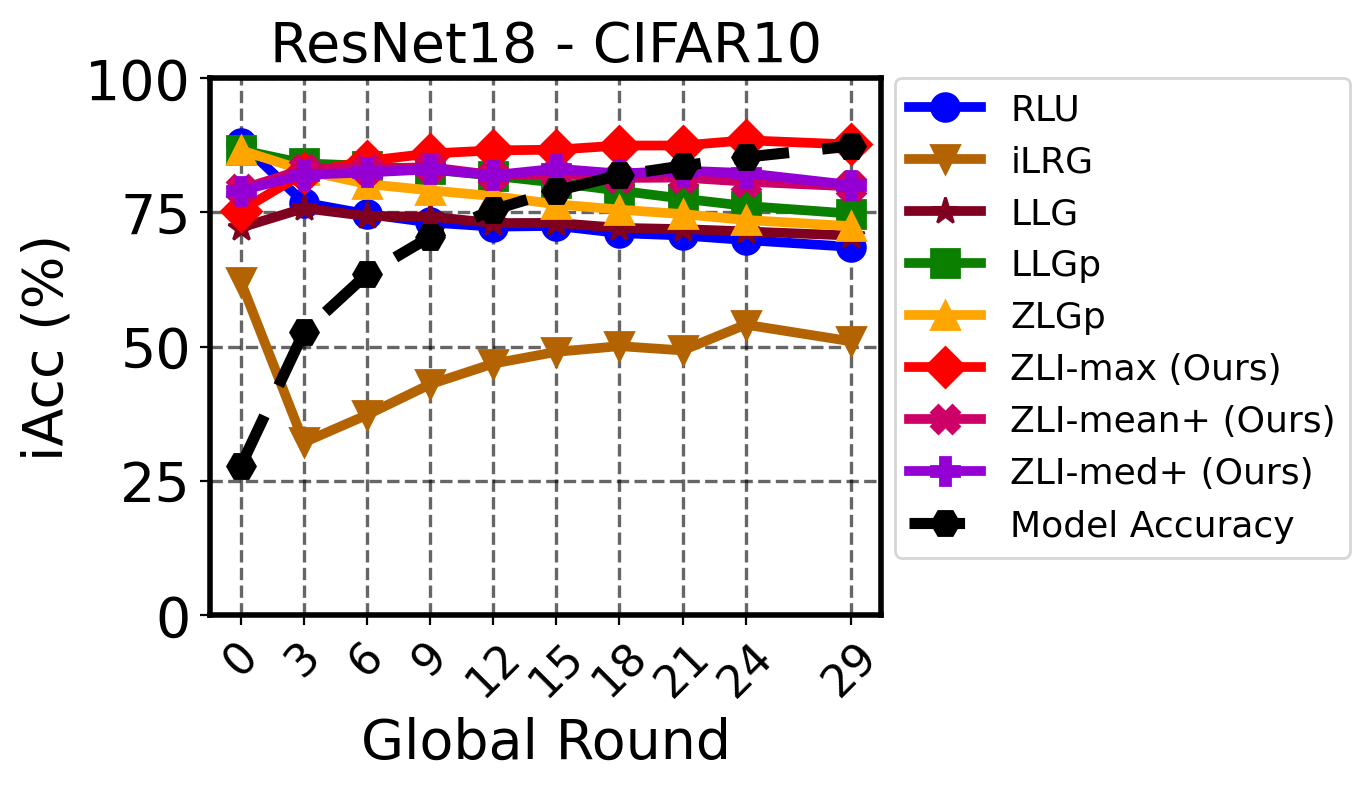
\includegraphics[width=\textwidth]{figures/fig1b_cifar10.png}
\caption{}
\label{fig:rq2-sweep-b}
\end{subfigure}
\hfill
\begin{subfigure}[b]{0.32\textwidth}
\centering
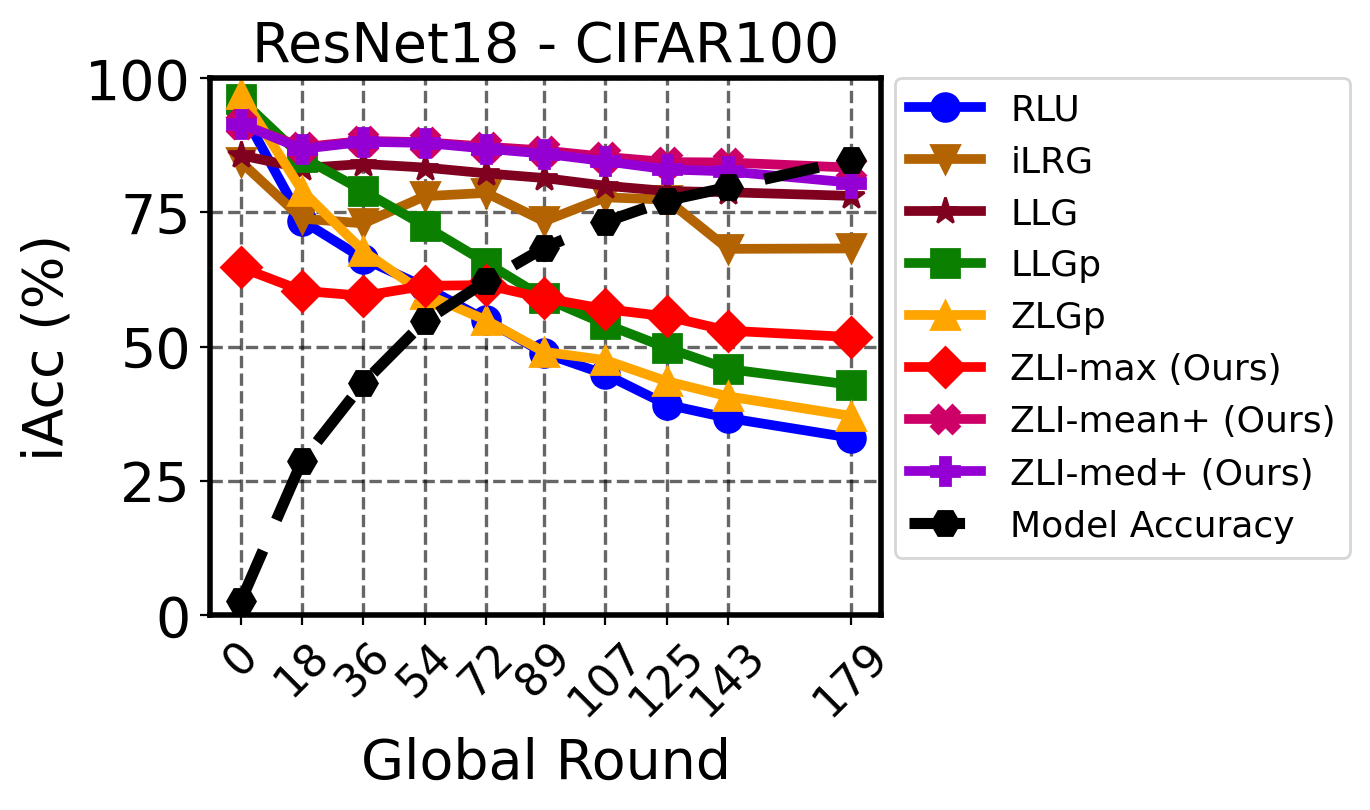
\includegraphics[width=\textwidth]{figures/fig1c_cifar100.png}
\caption{}
\label{fig:rq2-sweep-c}
\end{subfigure}
\caption{Instance-level recovery (irec, labelled iAcc on the axis) of
each attack as training progresses, drawn in the exact style of
\texttt{figure/Line\_chart.py}: the black dashed curve is the attacked
model's own training accuracy at that global round. \ourmethod{}'s three
variants (\texttt{max}, \texttt{mean+}, \texttt{med+},
Section~\ref{sec:method-gstar}) are plotted alongside the five
baselines; $m=10$ throughout (Table~\ref{tab:exhibits}).}
\label{fig:rq2-sweep}
\end{figure*}

Figure~\ref{fig:rq2-sweep} answers RQ2 across the full accuracy range
rather than only at convergence. On CIFAR-100 (panel c, $\alpha=0.1$,
most skewed), RLU and ZLG$^+$ fall from above $90\%$ at the first round to
$33$--$37\%$ at convergence, while \ourmethod{}'s \texttt{mean+} and
\texttt{med+} stay within $78$--$92\%$ across the entire sweep; LLG and
LLG$^+$ also degrade, though less sharply, and \texttt{max} declines
further than \texttt{mean+}/\texttt{med+} here, consistent with
Section~\ref{sec:method-gstar}'s stated trade-off at $\alpha=0.1$ (many
absent classes favor \texttt{mean+}/\texttt{med+}). On CIFAR-10 and SVHN
(panels a--b, $\alpha=0.5$, fewer absent classes) the separation is
smaller and \texttt{max} is competitive with or ahead of the other two
variants, again matching that same trade-off rather than contradicting
it. No baseline is uniformly best or uniformly worst across all three
panels; RLU in particular starts highest on two of the three datasets and
ends lowest on all three, the pattern Section~\ref{sec:eval-rq} calls out
as RQ1's prediction, not just a RQ2 comparison point.

\begin{table*}[t]
\centering
\caption{irec at a single, well-converged checkpoint per dataset/model
pair (Section~\ref{sec:eval-checkpoints}), at window length $m=10$ and
$m=1$ (Table~\ref{tab:exhibits}). Bold marks the best method per row.
\texttt{max}, \texttt{mean+}, \texttt{med+} are \ourmethod{}'s three
variants (Section~\ref{sec:method-gstar}).}
\label{tab:rq2-main}
\footnotesize
\setlength{\tabcolsep}{3pt}
\begin{tabular}{@{}l c c c c c c c c c c@{}}
\toprule
& & & \multicolumn{5}{c}{Baselines} & \multicolumn{3}{c}{\ourmethod{}} \\
\cmidrule(lr){4-8}\cmidrule(lr){9-11}
Dataset/Model & $\alpha$ & $m$ & iLRG & LLG & LLG$^+$ & ZLG$^+$ & RLU & \texttt{max} & \texttt{mean+} & \texttt{med+} \\
\midrule
\multirow{2}{*}{VGG16/CIFAR-10} & \multirow{2}{*}{0.5}
 & 10 & 0.292 & 0.777 & 0.671 & 0.720 & 0.779 & \textbf{0.804} & 0.801 & 0.801 \\
 & & 1 & 0.436 & 0.708 & 0.779 & \textbf{0.830} & 0.665 & 0.785 & 0.784 & 0.730 \\
\multirow{2}{*}{ResNet18/CIFAR-10} & \multirow{2}{*}{0.5}
 & 10 & 0.510 & 0.707 & 0.748 & 0.724 & 0.686 & \textbf{0.876} & 0.798 & 0.801 \\
 & & 1 & 0.510 & 0.702 & 0.850 & \textbf{0.855} & 0.686 & 0.815 & 0.786 & 0.746 \\
\multirow{2}{*}{ResNet18/CIFAR-100} & \multirow{2}{*}{0.1}
 & 10 & 0.683 & 0.781 & 0.429 & 0.371 & 0.330 & 0.518 & \textbf{0.834} & 0.805 \\
 & & 1 & 0.682 & 0.726 & 0.589 & 0.485 & 0.412 & 0.455 & \textbf{0.762} & 0.689 \\
\multirow{2}{*}{MobileNetV2/SVHN} & \multirow{2}{*}{0.5}
 & 10 & 0.484 & 0.707 & 0.707 & 0.536 & 0.586 & 0.764 & \textbf{0.772} & 0.747 \\
 & & 1 & 0.520 & 0.691 & 0.657 & 0.485 & 0.523 & 0.677 & \textbf{0.735} & 0.668 \\
\multirow{2}{*}{MobileNetV2/MNIST} & \multirow{2}{*}{0.5}
 & 10 & 0.602 & 0.696 & 0.687 & 0.637 & 0.632 & \textbf{0.869} & 0.781 & 0.794 \\
 & & 1 & 0.537 & 0.670 & 0.752 & 0.706 & 0.625 & \textbf{0.795} & 0.747 & 0.692 \\
\bottomrule
\end{tabular}
\end{table*}

Table~\ref{tab:rq2-main} fixes a single converged checkpoint per pair
(Section~\ref{sec:eval-checkpoints}) and reports both window lengths side
by side. Some version of \ourmethod{} is best in $8$ of the $10$ rows;
the two exceptions are both $\alpha=0.5$ (ResNet18/CIFAR-10 and
VGG16/CIFAR-10 at $m=1$), where ZLG$^+$ wins narrowly -- we do not smooth
over this, since a method that is uniformly best everywhere would itself
be a reason for suspicion. Three caveats on comparability, stated
precisely rather than left implicit: (i) RLU is the only estimator that
reads the learning rate (Section~\ref{sec:eval-attack}), and the $m=1$
and $m=10$ rows of three pairs (ResNet18/CIFAR-10, ResNet18/CIFAR-100,
MobileNetV2/MNIST) were run at different learning rates ($0.05$ vs.\
$0.01$), so RLU's two rows for those pairs are not a controlled
single-variable comparison; (ii) the VGG16/CIFAR-10 rows use two
different checkpoints ($86.75\%$ at $m=10$, $89.33\%$ at $m=1$), both
converged but not identical; (iii) the original (dummy-data) form of ZLG
has no corresponding attack implementation in this codebase yet
(\texttt{client/attacks.py} only implements \texttt{ZLGp\_attack}), so
only ZLG$^+$ appears in Figure~\ref{fig:rq2-sweep} and
Table~\ref{tab:rq2-main} for now; dummy-data ZLG is planned as a
follow-up run and will be added to both once available, which is what
makes Section~\ref{sec:related}'s "both forms" claim true. A fourth
method
(\texttt{VLI}, the precursor bias-sum attack read by \texttt{--scheme
All} and \texttt{Client\_prox.VLI}, distinct from \ourmethod{}'s closed
form) was run in every log underlying this table and is omitted here as
superseded by \ourmethod{}, not because it was dropped silently.

% ----------------------------------------------------------------------------
% Bibliography entry introduced by this file.
% ----------------------------------------------------------------------------
% @inproceedings{hsu2019dirichlet,
%   author    = {Hsu, Tzu-Ming Harry and Qi, Hang and Brown, Matthew},
%   title     = {Measuring the Effects of Non-Identical Data Distribution
%                for Federated Visual Classification},
%   booktitle = {arXiv:1909.06335},
%   year      = {2019}
% }
